\subsection{Diseño del barrido}

Se corrieron diez repeticiones independientes de cada uno de los cinco
kernels de calibración del catálogo (\texttt{stream\_official},
\texttt{ert\_probe} para CPU; \texttt{gpu\_stream\_bw},
\texttt{gpu\_ert\_probe\_fp32}, \texttt{gpu\_ert\_probe\_fp64} para GPU),
extrayendo el valor reportado por cada una directamente de su salida
estándar -- sin usar la orquestación completa de calibración
(\texttt{run\_calibration}/\texttt{run\_gpu\_calibration}), que normalmente
solo calibra una vez por campaña.

\subsection{Resultados}

La Figura~\ref{fig:calibration-dist} y la Tabla~\ref{tab:calibration-dist}
muestran la dispersión real de diez mediciones independientes de cada
referencia de calibración.

\begin{table}[H]
\centering
\caption{Dispersión de 10 calibraciones independientes.}
\label{tab:calibration-dist}
\begin{tabular}{@{}lrr@{}}
\toprule
\textbf{Kernel de calibración} & \textbf{CV\% (10 repeticiones)} & \textbf{Desviación vs. referencia declarada} \\
\midrule
\texttt{stream\_official} (BW, CPU) & 0{,}593\,\% & 0{,}10\,\% \\
\texttt{ert\_probe} (FLOPs, CPU) & 0{,}127\,\% & 0{,}23\,\% \\
\texttt{gpu\_stream\_bw} (BW, GPU) & 0{,}628\,\% & sin referencia declarada \\
\texttt{gpu\_ert\_probe\_fp32} (FLOPs, GPU) & 0{,}0012\,\% & sin referencia declarada \\
\texttt{gpu\_ert\_probe\_fp64} (FLOPs, GPU) & 0{,}000016\,\% & sin referencia declarada \\
\bottomrule
\end{tabular}
\end{table}

\begin{figure}[H]
\centering
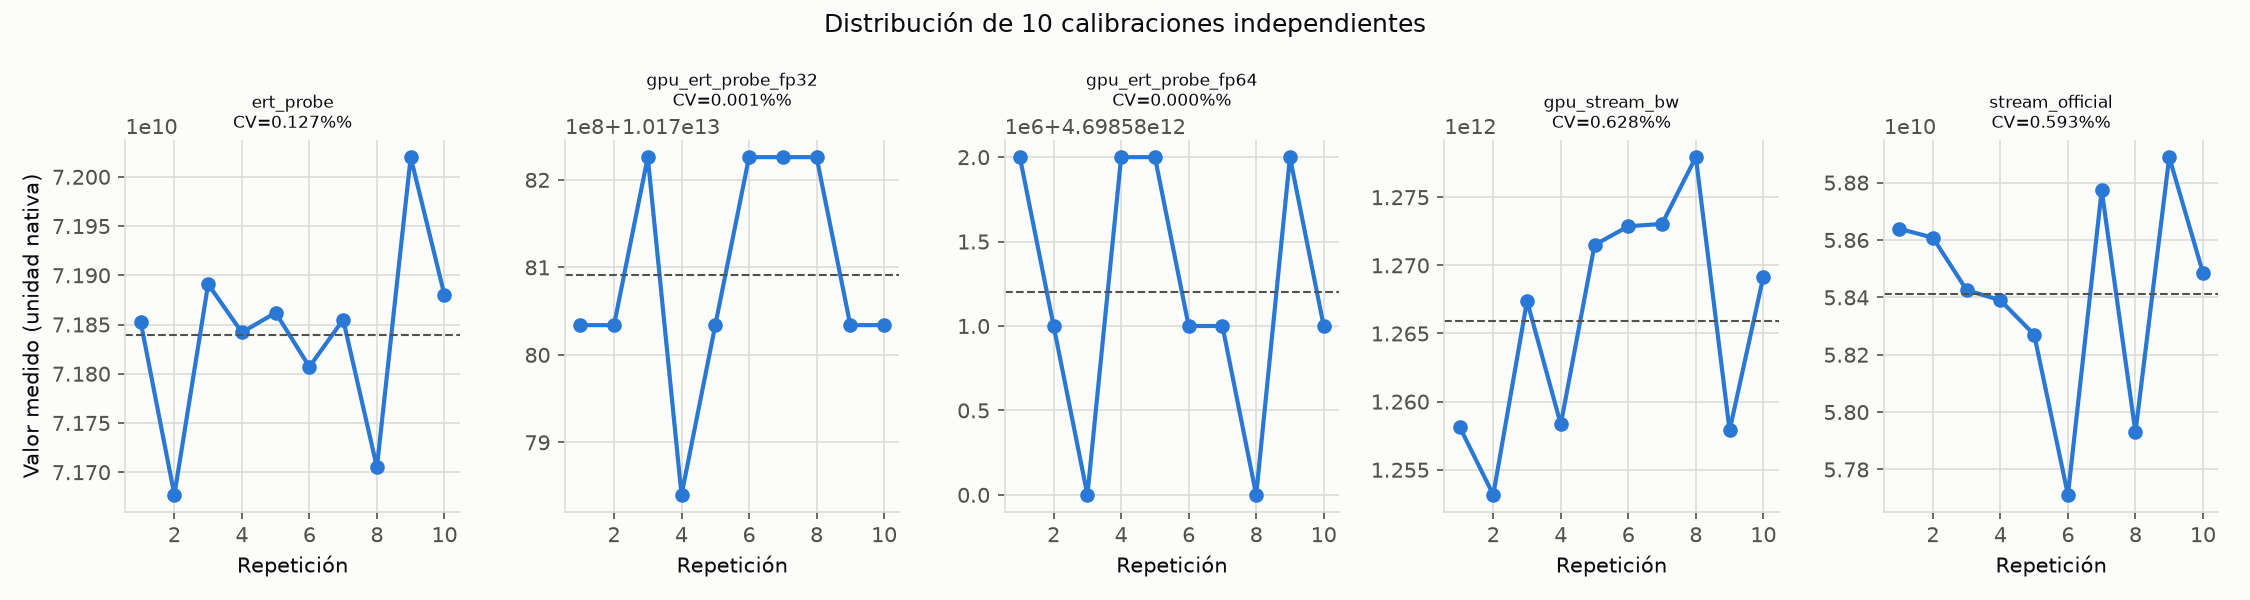
\includegraphics[width=\textwidth]{../plots/calibration_repeats/calibration_distribution.png}
\caption{Diez calibraciones independientes por kernel de referencia. La
línea punteada marca la media. Nótese la escala de cada panel: la
dispersión visual parece grande, pero el eje vertical cubre una fracción
mínima del valor absoluto en todos los casos.}
\label{fig:calibration-dist}
\end{figure}

Los probes de FLOPs de GPU (\texttt{gpu\_ert\_probe\_fp32/fp64}) muestran
una estabilidad extraordinaria (CV\% $<$0{,}002\,\%, y para FP64
0{,}000016\,\% -- esencialmente determinista) -- consistente con el
hallazgo ya documentado en el proyecto (ARC-77) de que la GPU no varía su
reloj bajo carga en este nodo: sin ninguna variabilidad de \textit{boost}
que introducir, el pico de cómputo medido es prácticamente determinista de
una corrida a otra. El ancho de banda (CPU y GPU) y el pico de FLOPs de CPU
muestran algo más de dispersión ($\sim$0{,}1--0{,}6\,\%), coherente con la
variabilidad normal de acceso a memoria compartida del sistema.

Es importante no sobreinterpretar lo que esta baja dispersión demuestra:
que el ruido normal esté en 0{,}1--0{,}6\,\% no dice nada sobre si 40\,\%
es un valor mejor que 10\,\%, 20\,\% o 30\,\% -- ninguno de esos valores
alternativos se comparó aquí. Lo que sí demuestra, y es la única
afirmación que este barrido respalda, es dónde está el ruido de fondo
real frente al cual cualquiera de esas tolerancias tendría que operar.

\textbf{Conclusión sobre \texttt{D03\_TOLERANCE\_FRACTION} (40\,\%, CPU)
-- \emph{guardarraíl conservador confirmado, no tolerancia derivada
estadísticamente}}: esta medición, independiente de la ya reportada en el
reporte anterior (una única calibración de referencia), confirma con diez
repeticiones que la desviación real de la calibración de CPU frente a su
valor de referencia (0{,}10\,\% y 0{,}23\,\%) está casi tres órdenes de
magnitud por debajo del 40\,\% configurado. Esto confirma que el 40\,\%
nunca se ha acercado a su límite en la práctica y que sigue funcionando
como red de seguridad contra errores groseros de configuración (el caso
histórico que la motivó, ARC-55, fue una discrepancia de más de
5$\times$) -- pero no confirma que 40\,\% sea el valor óptimo ni que esté
derivado del ruido medido; es, y debe reportarse como, un margen de
seguridad amplio y deliberadamente conservador, no una tolerancia
estadística ajustada al ruido real.

\textbf{Conclusión sobre la tolerancia cruzada de GPU (5\,\%, sin
datasheet) -- \emph{parcialmente justificada, pendiente de DVFS real}}:
esta medición establece una cota inferior útil -- el ruido de medición
puro de los probes de GPU (0{,}0004--0{,}63\,\%) es tan pequeño que, si una
futura calibración a un nivel de frecuencia distinto de REF mostrara una
diferencia cercana al 5\,\% de tolerancia, esa diferencia casi con toda
seguridad reflejaría un cambio real de frecuencia y no ruido de medición.
Pero esto es evidencia de que el 5\,\% tiene margen frente al ruido de
fondo, no evidencia de que el chequeo efectivamente detecte una aplicación
fallida de frecuencia cuando ocurra: esa verificación end-to-end (aplicar
un nivel de frecuencia real distinto de REF y confirmar que la calibración
cruzada lo detecta) sigue sin poder hacerse hasta que llegue el permiso
P4, y esta tolerancia debe seguir clasificada como parcial, no confirmada,
mientras eso no se verifique.
